\section{Stability}
After evaluating numerically the overall efficiency of the method for the one dimensional case, the theoretical and numerical stability will be studied. In fact, the theoretical stability does not lead to the stability of the numerical scheme. Therefore, both stabilities will be studied separately
\subsection{Theoretical stability}
\subsubsection{Well-posedness}
The definition of the well-posedness is that a problem is said to be well-posed if it has a solution, that should be unique and should depend continuously on the data of the problem. This last requirement states that perturbations such as errors in measurement should not affect the solution in a too large proportion. 


\subsection{Stability of the numerical method}
In order to prove the stability of the temporal scheme, we can recall the following result concerning integration methods \cite{Geradin}: An integration scheme is said to be stable if there exists an integration step $h_0 > 0$ so that for any $h \in [0, h_0]$, a finite variation of the state vector at time $t^n$ induces only a non-increasing variation of the state vector $q^{n+1}$ calculated at a subsequent instant $t^{n+1}$.\\
In our case we will study the stability of the scheme with the temporal discretization presented in part \ref{part:describ}. This reduces to the analysis of the stability properties of the Newmark-$\beta$ scheme used in the algorithm \ref{algo} for the PML uniquely. We will focus our attention of the stability of the temporal scheme applied on only one element. We can prove the stability on one element the result extends to the other element \cite{Belytschko}. First of all we need to go back to the equations of motion and define the state vector: $Q^n = [\dot{u}^n, u^n, H^n]^T$.
The objective is to define the matrices $A$ and $B$ such that:
\begin{equation}
    A(h) Q^{n+1} + B(h) Q^{n} = 0
    \label{eq:matrix_form}
\end{equation}
which is in fact the matrix form of the equations of motion. Since each component of the state vector have the size $2 \times 1$, the matrices $A$ and $B$ are $6 \times 6$. This formulation comes from the fact that the we used have only one bar element composed of two points.    
Let us first recall the equation of motion at time $t^n$ and $t^{n+1}$:
\begin{equation}
    M  \Ddot{u}^n = -C \Dot{u}^n - K u^n +p_{int}^n 
\end{equation}
\begin{equation}
    M \Ddot{u}^{n+1} = -C \Dot{u}^{n+1} - K u^{n+1} +p_{int}^{n+1} 
\end{equation}
Using the recurrence relationship described in the algorithm \ref{algo} from the Newmark scheme, we obtain:
\begin{equation}
    M \dot{u}^{n+1} = M\Dot{u}^{n} + h(1-\gamma)\left[ -C \Dot{u}^n - K u^n +p_{int}^n   \right] + \gamma h \left[ -C \Dot{u}^{n+1} - K u^{n+1} +p_{int}^{n+1} \right]
    \label{eq:rec1}
\end{equation}

\begin{equation}
    M u^{n+1} = M u^{n} + h M \dot{u}^n + h^2(\frac{1}{2}-\beta)\left[ -C \Dot{u}^n - K u^n +p_{int}^n   \right] + \beta h^2 \left[ -C \Dot{u}^{n+1} - K u^{n+1} +p_{int}^{n+1} \right]
    \label{eq:rec2}
\end{equation}
With $\beta$ and $\gamma$ the parameters of the Newmark scheme. We also have a recurrence relation for $H^{n+1}$. 
\begin{equation}
    H^{n+1} = H^n + h \epsilon^{n+1}
    \label{eq:rec3}
\end{equation}
With $\epsilon^{n+1}$ the strain at time $t^{n+1}$ which can be expressed in function of $u^{n+1}$ and $H^n$. The following formulation is element wise, since we consider the stability on only one element this formulation suffices:
\begin{equation}
    \epsilon^{{n+1}^e} = \frac{[B]\{u^{{n+1}^e}\} - \frac{c_s}{L_p} f^p_x H^n}{\alpha}
    \label{eq:eps}
\end{equation}
with $\alpha = (1+f^e_x)+\frac{c_s}{L_p} f^p_x $.\\ 
Using the equations \ref{eq:rec1}, \ref{eq:rec2} and \ref{eq:rec3}, we seek the definition of the matrix form \ref{eq:matrix_form}. We will define the matrices per blocs of size $2 \times 2$. In the following development the mass $M$, damping $C$ and stiffness $K$ matrices are using the formulas \ref{eq:me}, \ref{eq:ce} and \ref{eq:Ke} for one element.  \\
First of all, let us multiply by the left \ref{eq:rec1} and \ref{eq:rec2} by $M^{-1}$ and put all the terms to the left side:

\begin{multline}
    \dot{u}^{n+1}\left[I + \gamma h M^{-1}C\right] + u^{n+1}\left[\gamma h M^{-1}K \right] -\gamma h M^{-1} p_{int}^{n+1}  
    + \dot{u}^n\left[-I + h(1-\gamma)M^{-1}C   \right] \\+ u^n\left[ h(1-\gamma) M^{-1}K \right] - h(1-\gamma)M^{-1} p_{int}^n = 0
\end{multline}
\begin{multline}
    \dot{u}^{n+1}\left[\beta h^2 M^{-1} C \right] +  u^{n+1}\left[I+\beta h^2 M^{-1} K  \right] - \beta h^2 M^{-1} p_{int}^{n+1} + \dot{u}^n \left[ -h I + h^2(\frac{1}{2}-\beta) M^{-1} C \right] \\
    + u^n\left[-I + h^2(\frac{1}{2}-\beta) M^{-1} K \right] - h^2(\frac{1}{2}-\beta) M^{-1}p^n_{int}=0
\end{multline}
The only problem remaining before constructing the matrices $A(h)$ and $B(h)$ is how to handle the term of the internal forces $p_{int}$.
Let us recall its expression first:
\begin{equation}
    p_{int}^n = \int^{1}_{-1}[B]^T\frac{c_s}{L_p}\frac{f^p(\xi)}{\alpha(\xi)} H^n S  \frac{L_e}{2} d\xi
\end{equation}
Since we assumed that $f^p$ and $f^e$ are constant and using the quadrature to evaluate the integral with two Gauss points with weights $w=1$  we obtain

\begin{equation}
    p_{int}^n = \frac{c_s}{L_p} E S \begin{bmatrix} \frac{2}{L_e} \\ \frac{-2}{L_e} \end{bmatrix} \begin{bmatrix} 1 \times \frac{H_{n,k=1} f^p_{k=1}}{\alpha_{k=1}}&  1 \times \frac{H_{n,k=2} f^p_{k=2}}{\alpha_{k=2}}  \\ \end{bmatrix} = \frac{c_s}{L_p} E S \frac{f^p}{\alpha} \begin{bmatrix}
        1 &1\\
        -1 & -1
    \end{bmatrix} \begin{bmatrix}H_{n,k=1} \\ H_{n,k=2}\end{bmatrix}
\end{equation} 
where $k=1$ corresponds to the first Gauss point and $k=2$ to the second. We also have:
\begin{equation}
    A_p = \frac{c_s E S}{L_p}\frac{f^p_x}{\alpha} \begin{bmatrix}
        1 &1\\
        -1 & -1
    \end{bmatrix}
\end{equation}
For the last row of the matrices we need to focus on the equation:
\begin{equation}
    H^{n+1} = H^n + h \epsilon^{n+1}
\end{equation}
with $\epsilon^{n+1}$ given by the equation \ref{eq:eps} such that we obtain:
\begin{equation}
    H^{n+1}+H^n\left[-I + h \frac{c_s}{L_p} \frac{f^p_x}{\alpha} \right] - \frac{h}{\alpha} \left[\overline{B} \right]u^{n+1} 
\end{equation}
\begin{equation}
    A(h) = \begin{bmatrix} I+\gamma h M^{-1} C & \gamma h M^{-1} K & -\gamma h M^{-1} A_p \\
    \beta h^2 M^{-1} C & I+\beta h^2 M^{-1} K & -\beta h^2 M^{-1} A_p\\
    0 & -\frac{h}{\alpha} \overline{B} & I
    \end{bmatrix}
    \label{eq:A(h)}
\end{equation}
where 
\begin{equation}
    \overline{B} = \frac{1}{L_e} \begin{bmatrix}
        -1 & 1\\
        -1 & 1
    \end{bmatrix}
\end{equation}
We expressed in \ref{eq:A(h)} all the terms depending on time $t^{n+1}$, let us now express the remaining terms depending on time $t^n$:
\begin{equation}
    B(h) = \begin{bmatrix} -I+(1-\gamma) h M^{-1} C & (1-\gamma) h M^{-1} K & -(1-\gamma) h M^{-1} A_p \\
    -h I + (\frac{1}{2}-\beta) h^2 M^{-1} C & -I+(\frac{1}{2}-\beta) h^2 M^{-1} K & -(\frac{1}{2}-\beta) h^2 M^{-1} A_p\\
    0 & 0 & -I+\frac{c_s}{L_p}\frac{f^p_x}{\alpha} I
    \end{bmatrix}
    \label{eq:B(h)}
\end{equation}
Using the equation \ref{eq:A(h)} and \ref{eq:B(h)}, we can define the amplification matrix associated with the integration operator $H(h) = A(h)^{-1} B(h)$.\\
As shown in \cite{Geradin}, the stability of the integration method is ensured if the eigenvalues of the amplification matrix $H(h)$ are contained in the unit circle i.e.\ the moduli of the eigenvalues are lower than unity.\\ To prove the stability of our temporal scheme let us consider the simplest case where $f^e_x = 0$ everywhere and $f^p_x$ is a constant equals to $10$. Let us also consider the case of the unconditionally stable Newmark scheme ie $\beta = 0.25$ and $\gamma = 0.5$. We will consider several values of time steps and for each of them we will plot the eigenvalues of the amplification matrix in the complex plane. For $h$ taking its value from $0.001$ to $10$ by step of $0.001$ we obtain the following figure:
\begin{figure}[H]
    \centering
    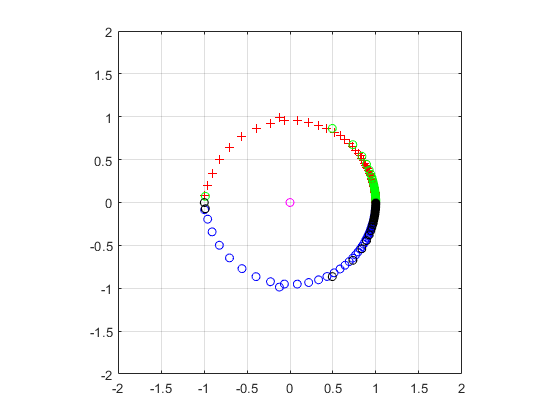
\includegraphics[scale=0.6]{images/radius.png}
    \caption{Eigenvalues of the amplification matrix in the complex plane}
    \label{fig:eigenval_amp}
\end{figure}
As we can observe on figure \ref{fig:eigenval_amp}, the eigenvalues of the amplification matrix $H(h)$ for different values of $h$ remain in the unit circle. When $h$ increases the eigenvalues are positioned at the left of the unit circle. For small values of $h$ the eigenvalues are at the right. For more complex case including those where the attenuation function are not assumed constant this result holds. This result ensures that the temporal integration scheme , we developed is stable in time for the one dimensional PML. This result shows that the integration scheme derived from the equation of the PML is stable in time. \\
In order to evaluate the properties of a numerical scheme in terms of stability, an interesting method is to look at the spectral radius, the periodicity error and the numerical damping. The spectral radius of the method is given by the modulus of the highest eigenvalue:
\begin{equation}
    R(A) = \max_i(|\lambda_i|)
\end{equation}
We will express this parameter in function of $\Omega = \omega h$ where $\omega = \sqrt{\frac{k}{m}}$ and $k=\frac{E S}{L_p}$. $m$ is the mass of the bar (in our case just an element). The asymptotic value of the spectral radius for $\omega h \rightarrow \infty$ gives an information about the stability of the method over the entire frequency domain.
\begin{figure}[H]
    \centering
    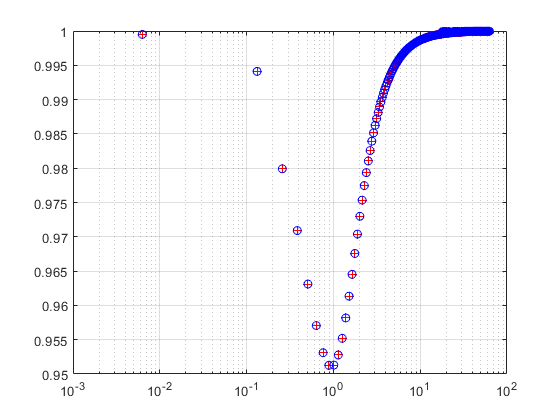
\includegraphics[scale=0.6]{images/spectral_rad.png}
    \caption{Spectral radius in function of $h\omega$}
    \label{fig:spectral_rad}
\end{figure}
As shown on the figure \ref{fig:spectral_rad}, the spectral radius remains under the value $1$ and its asymptotic value tends to $1$ as  $\omega h \rightarrow \infty$. This demonstrates that the numerical scheme is stable over the entire frequency domain. 
Let us now focus on the periodicity error which results from the comparison between the numerical and the exact frequencies obtained for the one degree-of-freedom oscillator:
\begin{equation}
    \frac{\Delta T}{T} = \frac{\omega h}{ \phi} - 1 \hspace{2cm}\textnormal{where} \hspace{1cm} \phi=tan^{-1}\left(\frac{\operatorname{Im} \lambda_1}{\operatorname{Re} \lambda_1}  \right)
    \label{eq:period_err}
\end{equation}
Therefore this is a measurement of the frequency distortion for each eigenfrequency in the model. 

\begin{figure}[H]
    \centering
    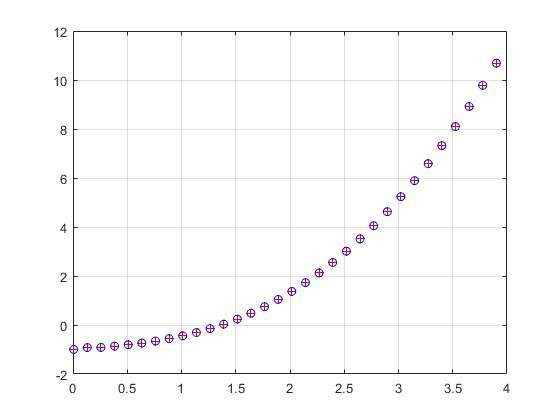
\includegraphics[scale=0.6]{images/relative_periodicity_error.png}
    \caption{relative periodicity error in function of $h\omega$}
    \label{fig:relative_per_err}
\end{figure}
As observed in \ref{fig:relative_per_err}, the relative periodicity error increases with $h \omega$ looking back at the equation \ref{eq:period_err} and knowing that the modulus of each eigenvalue is smaller or equal to $1$, the result obtained here about the relative periodicity error is the one expected. Since this result is difficult to interpret a more complete analysis will be done in the next report. Indeed some questions remain unanswered such as why the distortion at $h=0$ is different than $0$ or other questions about the numerical damping ratio we will present now. \\
The last parameter to be investigate is the numerical damping ratio. It compare the time decay coefficient of the real part of the solution to the numerical frequency.
\begin{equation}
    \xi = -\frac{log(|\lambda_1|)}{\phi}
    \label{eq:num_damp}
\end{equation}
It measures the percentage of critical damping introduced in the system by the integration operator. In fact it is expected to damped out the high frequencies introduced by the time integration operator.   
\begin{figure}[H]
    \centering
    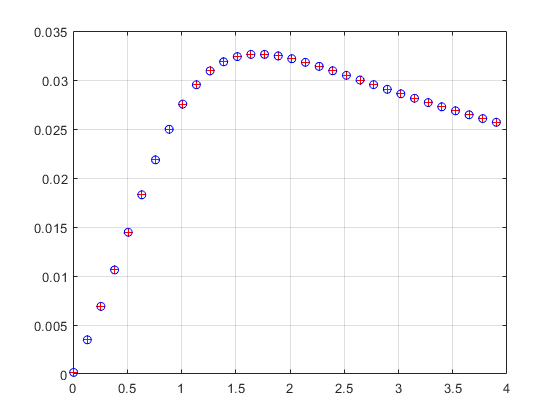
\includegraphics[scale=0.6]{images/Numerical_damping_ratio.png}
    \caption{Numerical damping ratio in function of $h\omega$}
    \label{fig:num_damp_ratio}
\end{figure}
In order to compare the results obtained on the Newmark-$\beta$ unconditionally stable scheme, let us make the same analysis of stability on the Newmark explicit temporal integration scheme for the PML with $\beta=0$ and $\alpha=0.5$ (central differences). 
\begin{figure}[H]
\centering
\begin{minipage}[b]{0.475\textwidth}
    \centering
    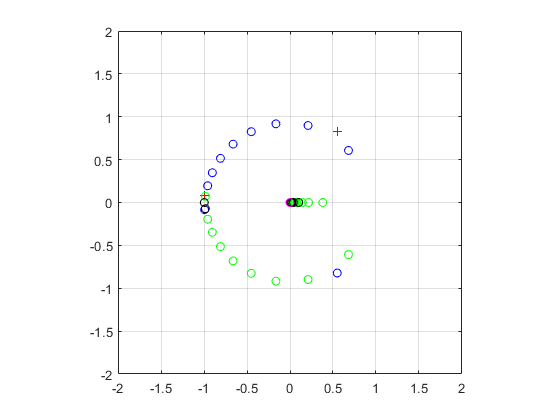
\includegraphics[width=\textwidth]{images/pml_expl_eig.png}
    \caption[Network2]%
    {{\small Eigenvalues in the complex plane}}    
    \label{fig:med_eig}
\end{minipage}
\hfill
\begin{minipage}[b]{0.475\textwidth}  
    \centering 
    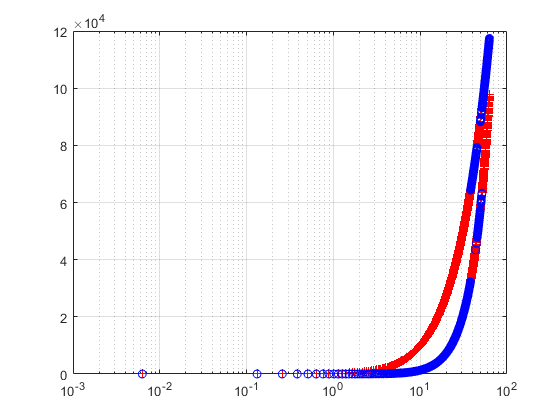
\includegraphics[width=\textwidth]{images/spectre_expl.png}
    \caption[]%
    {{\small Spectral radius in function of $h\omega$}}    
    \label{fig:med_spectre}
\end{minipage}
\vskip\baselineskip
\begin{minipage}[b]{0.475\textwidth}   
    \centering 
    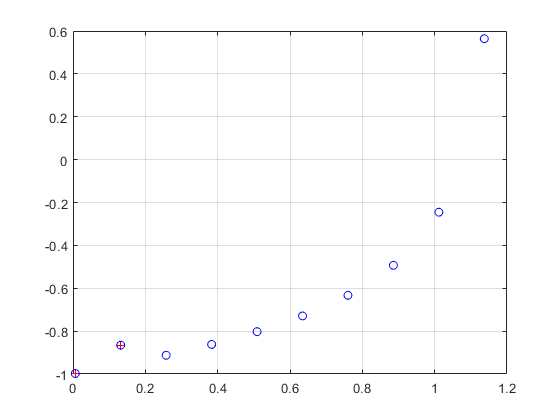
\includegraphics[width=\textwidth]{images/pml_exp_per.png}
    \caption[]%
    {{\small relative periodicity error in function of $h\omega$}}    
    \label{fig:med_relat_per}
\end{minipage}
\quad
\begin{minipage}[b]{0.475\textwidth}   
    \centering 
    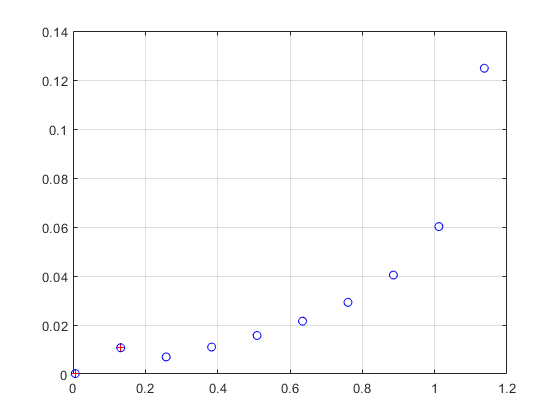
\includegraphics[width=\textwidth]{images/pml_expl_damp.png}
    \caption[]%
    {{\small Numerical damping ratio in function of $h\omega$}}    
    \label{fig:med_damp}
\end{minipage}
\end{figure}
As expected for a conditionally stable scheme, passed a certain value of $h \omega$ the scheme becomes unstable. This limit of stability is evaluated $h \omega = 2$ corresponding to the CFL condition.\\
We can also look at the behaviour of the Newmark explicit time integrator on the physical medium. In this case the equation of motion are the same as in a classic elastodynamic problem. In the following equation the state vector $q$ will be defined by $q^n=[\dot{u}^n, u^n]^T$. THe equation of motion at time $t^n$ and $t^{n+1}$ are:
\begin{equation}
\begin{aligned}
    M  \Ddot{u}^n &= -C \Dot{u}^n - K u^n +p^n  \\
    M \Ddot{u}^{n+1} &= -C \Dot{u}^{n+1} - K u^{n+1} +p^{n+1} 
\end{aligned}
\end{equation}
And taking into account the recurrence relationship given by the Newmark method:
\begin{equation}
\begin{aligned}
    M \dot{u}^{n+1} &= M\Dot{u}^{n} + h(1-\gamma)\left[ -C \Dot{u}^n - K u^n +p^n   \right] + \gamma h \left[ -C \Dot{u}^{n+1} - K u^{n+1} +p^{n+1} \right] \\
    M u^{n+1} &= M u^{n} + h M \dot{u}^n + h^2(\frac{1}{2}-\beta)\left[ -C \Dot{u}^n - K u^n +p^n   \right] + \beta h^2 \left[ -C \Dot{u}^{n+1} - K u^{n+1} +p^{n+1} \right]
\end{aligned}
\label{eq:med_rec}
\end{equation}
Therefore we can define the matrix form of this recurrence:
\begin{equation}
    q^{n+1} = A(h) q^n + g^{n+1}(h)
\end{equation}
The component of this relation can be defined using the equations \ref{eq:med_rec}. We obtain:
\begin{equation}
    A(h) = \begin{bmatrix}M+\gamma h C & \gamma h K \\ \beta h^2 C & M+ \beta h^2 K   \end{bmatrix}^{-1} \begin{bmatrix}(1-\gamma)hC-M& (1-\gamma)hK \\ (\frac{1}{2}-\beta)h^2C-hM& (\frac{1}{2}-\beta)h^2K-M \end{bmatrix} 
\end{equation}
and where
\begin{equation}
    g^{n+1}=\begin{bmatrix}M+\gamma h C & \gamma h K \\ \beta h^2 C & M+ \beta h^2 K   \end{bmatrix}^{-1} \begin{bmatrix}(1-\gamma)h p^n+\gamma h p^{n+1} \\ (\frac{1}{2}-\beta)h^2p^n+\beta h^2 p^{n+1}  \end{bmatrix}
\end{equation}
The matrix $A(h)$ is the matrix of amplification, its eigenvalues represents the normal vibration modes of the one dimensional element considered. Since the physical medium was assumed to have no damping $C=0$. Let us now expend the solution with respect to the eigenmodes of the structure. The equations of motion can be reduced to uncoupled normal equations:
\begin{equation}
    \Ddot{\eta}^n = - \omega \eta^n+\phi^n
\end{equation}
where $\phi^n$ is the participation factor at the excitation at time $t^n$. Thus using this system of uncoupled equations we can redifine the amplification matrix by:
\begin{equation}
    A(h) = \begin{bmatrix} 1& \gamma h \omega^2\\ 0&1+\beta h^2 \omega ^2\end{bmatrix}^{-1} \begin{bmatrix} 1& -(1-\gamma) h \omega^2\\ h&1-(\frac{1}{2}-\beta) h^2 \omega ^2\end{bmatrix}
\end{equation}
Using this definition of the amplification matrix, we can do the same analysis for the physical medium than the one done of the implicit Newmark scheme on the PML.
\begin{figure}[H]
\centering
\begin{minipage}[b]{0.475\textwidth}
    \centering
    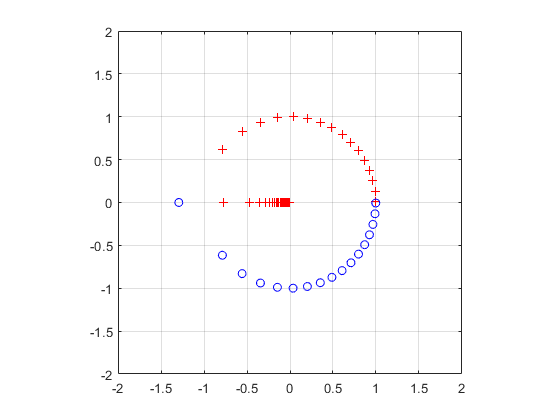
\includegraphics[width=\textwidth]{images/med_rad.png}
    \caption[Network2]%
    {{\small Eigenvalues in the complex plane}}    
    \label{fig:med_eig}
\end{minipage}
\hfill
\begin{minipage}[b]{0.475\textwidth}  
    \centering 
    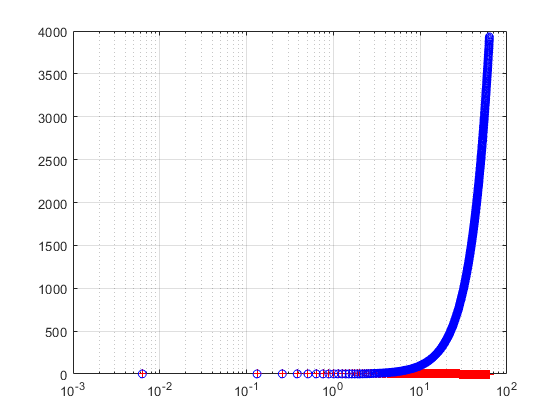
\includegraphics[width=\textwidth]{images/med_spectre.png}
    \caption[]%
    {{\small Spectral radius in function of $h\omega$}}    
    \label{fig:med_spectre}
\end{minipage}
\vskip\baselineskip
\begin{minipage}[b]{0.475\textwidth}   
    \centering 
    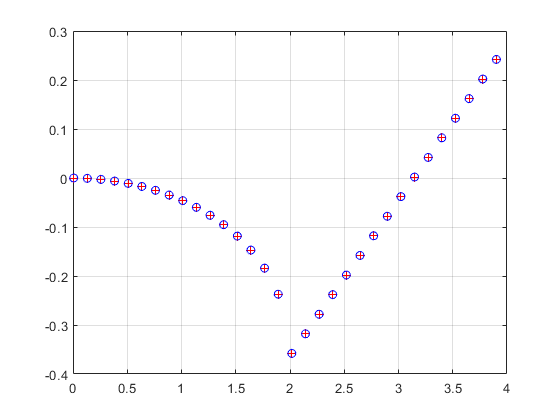
\includegraphics[width=\textwidth]{images/med_period.png}
    \caption[]%
    {{\small relative periodicity error in function of $h\omega$}}    
    \label{fig:med_relat_per}
\end{minipage}
\quad
\begin{minipage}[b]{0.475\textwidth}   
    \centering 
    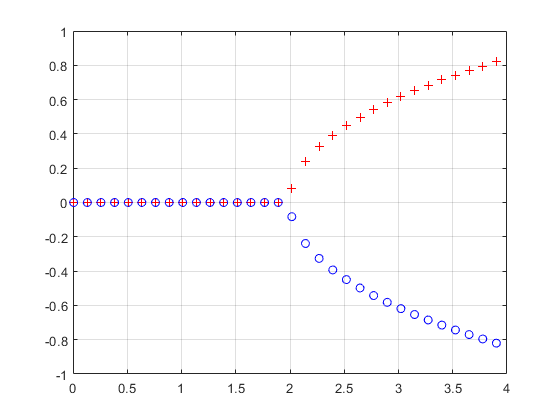
\includegraphics[width=\textwidth]{images/med_damp.png}
    \caption[]%
    {{\small Numerical damping ratio in function of $h\omega$}}    
    \label{fig:med_damp}
\end{minipage}
\end{figure}
We can observe on the figure \ref{fig:med_eig} that for a certain value of $h$ the eigenvalues seems to exit the unit circle. This is the proof that at a certain point the scheme becomes unstable and amplified drastically even small perturbations. This change from stable to unstable occurs when $h\omega > 2$ as we can see on the other figures




